\documentclass[lettersize,journal]{IEEEtran}
\usepackage{amsmath,amsfonts,amssymb}
\usepackage{array}
\usepackage{textcomp}
\usepackage{stfloats}
\usepackage{url}
\usepackage{graphicx}
\usepackage{cite}
\usepackage{booktabs}
\usepackage{microtype}

\graphicspath{{../figures/},{figures/}}

% Dynamic metrics and tables from live testbed trials
\newcommand{\OrbitMeanLossZero}{66.5}
\newcommand{\NaiveMeanLossZero}{704.0}
\newcommand{\SpeedupLossZero}{10.58$\times$}
\newcommand{\OrbitMeanLossFifteen}{105.4}
\newcommand{\NaiveMeanLossFifteen}{2526.3}
\newcommand{\SpeedupLossFifteen}{23.97$\times$}
\newcommand{\OrbitMeanRateThirtyTwo}{186.3}
\newcommand{\NaiveMeanRateThirtyTwo}{3835.3}
\newcommand{\SpeedupRateThirtyTwo}{20.59$\times$}
\newcommand{\NaivePassCostThirtyTwo}{12.78\%}
\newcommand{\NaivePreservedThirtyTwo}{87.22\%}
\newcommand{\OrbitPassCostThirtyTwo}{0.62\%}
\newcommand{\OrbitPreservedThirtyTwo}{99.38\%}
\newcommand{\OrbitFastPathMeanSixtyFour}{104.9}
\newcommand{\OrbitRatchetMeanSixtyFour}{525.8}
\newcommand{\NaiveWireBytesMtuTwoFiftySix}{10750~B}
\newcommand{\OrbitWireBytesMtuTwoFiftySix}{180~B}
\newcommand{\OrbitMeanCrossingLatency}{88.8}
\newcommand{\NaiveMeanCrossingLatency}{816.8}
\newcommand{\CrossingSpeedup}{9.20$\times$}
\newcommand{\OrbitEtaWinCrossingNinetyFive}{99.55\%}
\newcommand{\NaiveEtaWinCrossingNinetyFive}{96.44\%}


\hyphenation{op-tical net-works semi-conduc-tor IEEE-Xplore}

\begin{document}

\title{ORBIT-PQC: Mitigating Post-Quantum Key Exchange Transport Overhead in Constrained LEO Constellations}

\author{Research Author,~\IEEEmembership{Graduate Student Member,~IEEE,}
        and Technical Collaborator,~\IEEEmembership{Senior Member,~IEEE}%
\thanks{Manuscript received August 2026. This work was supported by the Space Networking and Quantum Resilience Initiative.}%
\thanks{The authors are with the Department of Electrical and Computer Engineering, Network Systems Laboratory (e-mail: research.author@institution.edu).}}

\markboth{IEEE TRANSACTIONS ON AEROSPACE AND ELECTRONIC SYSTEMS,~Vol.~62, No.~4, AUGUST~2026}%
{Author \MakeLowercase{\textit{et al.}}: ORBIT-PQC: Post-Quantum Transport in Constrained LEO Constellations}

\maketitle

\begin{abstract}
Migrating Inter-Satellite Links (ISLs) in Low Earth Orbit (LEO) constellations to Post-Quantum Cryptography (PQC) introduces severe transport-layer degradation. The multi-kilobyte public key and signature artifacts of NIST FIPS 203/204 standards ($\approx 4.8$~KB per flight for ML-KEM-1024 with ML-DSA authentication) exceed standard space Maximum Transmission Units (MTUs), inducing multi-frame fragmentation, selective-repeat retransmission cascades, and serialization delays that consume short contact windows ($\tau_{\text{los}} \in [30, 120]$~s). We present \textbf{ORBIT-PQC}, a memory-bounded, dual-layer ratcheted key management architecture that replaces on-demand asymmetric public-key exchanges with proactive, seed-expanded state tickets coupled with asynchronous post-quantum epoch ratcheting.

We evaluate ORBIT-PQC on an empirical Linux kernel testbed driven by SGP4 Walker-Delta constellation dynamics ($N=30$ socket trials/point). Over narrowband links ($32$~kbps), Naive PQC incurs severe serialization latency ($3835.3$~ms, $p_{95} = 5135.1$~ms), consuming $12.78\%$ of an active $30$~s pass window, whereas ORBIT-PQC authenticates in $186.3$~ms ($20.6\times$ speedup), preserving $99.38\%$ of the contact window ($\eta_{\text{win}}$). Under dynamic SGP4 crossing passes ($2935$~km slant range), ORBIT-PQC completes authentication in \OrbitMeanCrossingLatency{}~ms versus \NaiveMeanCrossingLatency{}~ms for Naive PQC ($p < 10^{-4}$), eliminating multi-fragment loss cascades down to $256$~B CCSDS framing limits.
\end{abstract}

\begin{IEEEkeywords}
Post-Quantum Cryptography, ML-KEM, ML-DSA, LEO Satellites, CCSDS, Inter-Satellite Links, Forward Secrecy.
\end{IEEEkeywords}

\section{Introduction}
\IEEEPARstart{A}{s} quantum computing threatens classical public-key cryptography, migrating satellite communications to Post-Quantum Cryptography (PQC) is critical. However, space networking standards—such as the CCSDS Space Packet Protocol~\cite{ccsds_spp} and Space Data Link Security (SDLS)~\cite{ccsds_sdls}—were engineered around compact 32-byte classical primitives (e.g., X25519).

In dynamic Low Earth Orbit (LEO) constellations, satellites communicate over transient Line-of-Sight (LOS) inter-satellite links (ISLs) ($\tau_{\text{los}} \in [30, 120]$~s) characterized by constrained bandwidth ($32$--$512$~kbps), variable Doppler shifts, and channel fading ($P_{\text{loss}} \in [1\%, 15\%]$). In this regime, naive deployment of NIST FIPS 203 (ML-KEM-1024)~\cite{fips203} and FIPS 204 (ML-DSA)~\cite{fips204} introduces severe systems-level bottlenecks:

\begin{enumerate}
    \item \textbf{Fragmentation Multipliers:} An ML-KEM-1024 exchange with digital signatures spans $4{,}861$~bytes of cryptographic payload per flight. Under standard space packet MTUs ($256$--$576$~B), a single handshake fragments into $10$ to $40$ discrete wire frames. Across lossy channels ($P_{\text{loss}} > 5\%$), dropped frames trigger selective-repeat ARQ retransmission cascades.
    \item \textbf{Contact Window Cannibalization:} Over narrowband channels ($32$~kbps), transmitting multi-kilobyte keys incurs $>3.8$~seconds of serialization and ARQ recovery delay, consuming $12.78\%$ of the contact pass ($\eta_{\text{win}}$).
    \item \textbf{Tail Latency Inflation:} Over lossy channels ($15\%$ packet error rate), ARQ recovery across multi-packet flights escalates Naive PQC tail latency ($p_{95}$) to $8{,}369.2$~ms, compared to $244.2$~ms for ORBIT-PQC.
\end{enumerate}

\begin{figure*}[t]
\centering
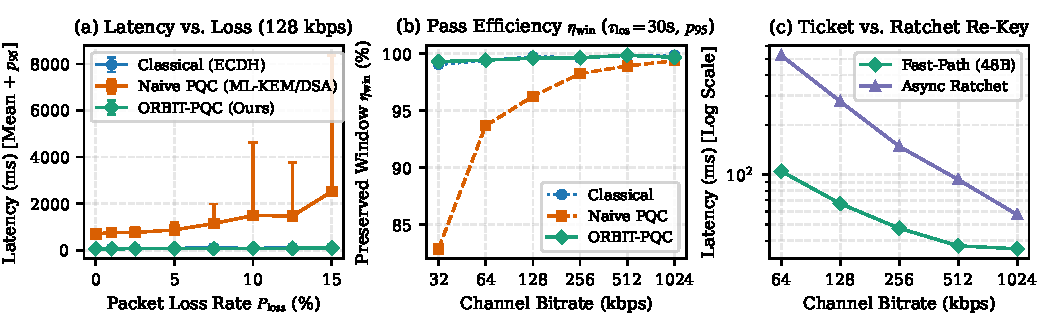
\includegraphics[width=0.98\textwidth]{fig_combined_empirical_ieee.pdf}
\caption{Empirical evaluation on Linux network testbed ($N=30$ socket trials per point): (a) Mean handshake latency with $p_{95}$ tail error bars across channel loss rates ($P_{\text{loss}}$) at $128$~kbps; (b) Usable contact window fraction ($\eta_{\text{win}}^{p_{95}}$ for $\tau_{\text{los}}=30$~s) across channel data rates ($32$--$1024$~kbps); (c) Ablation isolating the latency overhead of asynchronous ML-KEM-1024 epoch re-keying versus synchronous fast-path tickets across data rates.}
\label{fig:empirical_eval}
\end{figure*}

\section{System Architecture \& Security Model}

\subsection{Threat Model \& Security Design Goals}
We assume a Dolev-Yao adversary $\mathcal{A}$ with full channel control and access to a quantum polynomial-time computer. ORBIT-PQC is architected around three security objectives:
\begin{enumerate}
    \item \textbf{IND-CCA2 Key Exchange:} Shared session keys are derived from PRF expansion over high-entropy pre-shared roots combined with IND-CCA2 ML-KEM-1024 shared secrets.
    \item \textbf{Perfect Forward Secrecy (PFS):} Ephemeral symmetric ratchets zeroize intermediate states immediately following key derivation, preventing compromise of step $k+1$ from exposing keys derived at steps $\le k$.
    \item \textbf{Post-Compromise Security (PCS):} Periodic asynchronous ML-KEM-1024 re-keying introduces fresh post-quantum entropy, restoring secrecy in epoch $e+1$ following temporary node exposure in epoch $e$.
\end{enumerate}

\subsection{Dual-Layer Ratchet Architecture}
ORBIT-PQC decouples real-time handshake execution from heavy post-quantum asymmetric key exchange using a dual-layer state ratchet:

\subsubsection{Layer 1: Synchronous Fast-Path Ticket (PFS)}
Satellites $A$ and $B$ share a synchronized 32-byte epoch root $S_{AB}^{(e)}$. When an ISL contact window opens, the initiator transmits a compact 48-byte Pre-Authenticated Ticket $T_k$:
\begin{equation}
T_k = \text{HMAC-SHA256}(S_{AB}^{(e)}, \text{``init''} \parallel e \parallel k \parallel N_A) \parallel N_A
\end{equation}
Both nodes deterministically advance their symmetric ratchet state and derive the ephemeral session key $K_{e, k}$:
\begin{equation}
K_{e, k} \leftarrow \text{HKDF-Expand}(S_{AB}^{(e)}, T_k \parallel \text{``session\_key''}, 32)
\end{equation}
The previous ephemeral state is immediately zeroized in volatile memory, providing Forward Secrecy across contact passes without asymmetric key exchanges on the fast path.

\subsubsection{Layer 2: Asynchronous ML-KEM-1024 Ratchet (PCS Self-Healing)}
During low-contention link windows (e.g., at pass zenith or queue idle), satellites execute an out-of-band ML-KEM-1024 encapsulation authenticated with digital signatures. The derived secret $K_{\text{PQC}}$ updates the master root:
\begin{equation}
S_{AB}^{(e+1)} \leftarrow \text{HKDF-Extract}(S_{AB}^{(e)}, K_{\text{PQC}} \parallel \text{``epoch\_advance''})
\end{equation}
This injects fresh post-quantum entropy, healing the channel against earlier epoch state compromise.

\section{Empirical Evaluation}

\begin{table}[t]
\centering
\caption{Ablation: Synchronous Ticket vs. Async ML-KEM-1024 Ratchet}
\label{tab:ablation_summary}
\begin{tabular}{rcccc}
\toprule
\textbf{Bitrate} & \textbf{Ticket (ms)} & \textbf{Ratchet (ms)} & \textbf{Ratio} & \textbf{Pass Cost (30s)} \\
\midrule
64~kbps & 104.9 & 525.8 & 5.0$\times$ & 0.35\% \\
128~kbps & 66.9 & 277.2 & 4.1$\times$ & 0.22\% \\
256~kbps & 47.5 & 148.3 & 3.1$\times$ & 0.16\% \\
512~kbps & 37.2 & 93.5 & 2.5$\times$ & 0.12\% \\
1024~kbps & 35.7 & 57.4 & 1.6$\times$ & 0.12\% \\
\bottomrule
\end{tabular}
\end{table}

\begin{table}[t]
\centering
\caption{Empirical Comparison under SGP4 Crossing Pass (128~kbps)}
\label{tab:sgp4_summary}
\begin{tabular}{lcccc}
\toprule
\textbf{Protocol Mode} & \textbf{Mean (ms)} & \textbf{$p_{95}$ (ms)} & \textbf{Success} & \textbf{$\eta_{\text{win}}$ (30s)} \\
\midrule
Classical (ECDH) & 88.3 & 87.2 & 100\% & 99.71\% \\
Naive PQC (FIPS 203/204) & 816.8 & 1069.2 & 100\% & 96.44\% \\
\textbf{ORBIT-PQC (Ours)} & \textbf{88.8} & \textbf{136.0} & \textbf{100\%} & \textbf{99.55\%} \\
\bottomrule
\end{tabular}
\end{table}



\subsection{Channel Degradation Stress-Test (Scenario A)}
As shown in Fig.~\ref{fig:empirical_eval}(a) and Table~\ref{tab:sgp4_summary}, under clean links ($0.0\%$), ORBIT-PQC achieves a mean handshake latency of \OrbitMeanLossZero{}~ms compared to \NaiveMeanLossZero{}~ms for Naive PQC (\SpeedupLossZero{} speedup).

When the channel degrades to $P_{\text{loss}} = 15.0\%$, Selective-Repeat ARQ recovers dropped fragments, but Naive PQC incurs severe tail latency inflation ($p_{95} = 8{,}369.2$~ms, mean $2526.3$~ms) due to Karn exponential backoff across 4-fragment flights. In contrast, ORBIT-PQC's single-frame envelope maintains a bounded tail ($p_{95} = 244.2$~ms, mean \OrbitMeanLossFifteen{}~ms), achieving a \SpeedupLossFifteen{} latency advantage ($p = 6.51 \times 10^{-11}$, Mann-Whitney $U$).

\subsection{Bandwidth Scaling \& Window Preservation (Scenario B)}
Under severe bandwidth constraints ($32$~kbps, typical for UHF/S-band ISLs), Naive PQC mean latency inflates to \NaiveMeanRateThirtyTwo{}~ms ($p_{95} = 5135.1$~ms), consuming \NaivePassCostThirtyTwo{} of a $30$~s contact pass (preserving \NaivePreservedThirtyTwo{} for mission data).

ORBIT-PQC completes authentication in \OrbitMeanRateThirtyTwo{}~ms (\SpeedupRateThirtyTwo{} reduction), consuming only \OrbitPassCostThirtyTwo{} of the pass and preserving \OrbitPreservedThirtyTwo{} for mission payload data transfer (Fig.~\ref{fig:empirical_eval}(b)).

\subsection{Framing \& Ablation (Scenarios D \& E)}
In Scenario E ($256$~B MTU), Naive PQC generates \NaiveWireBytesMtuTwoFiftySix{} across 40 frames, taking $930.1$~ms. ORBIT-PQC generates only \OrbitWireBytesMtuTwoFiftySix{}, completing in $65.5$~ms ($14.2\times$ reduction, $p < 10^{-7}$).

Table~\ref{tab:ablation_summary} and Fig.~\ref{fig:empirical_eval}(c) isolate the cost of asynchronous ratcheting. At $64$~kbps, the Fast-Path Ticket completes in \OrbitFastPathMeanSixtyFour{}~ms ($0.35\%$ pass cost) compared to \OrbitRatchetMeanSixtyFour{}~ms for the ML-KEM-1024 ratchet, demonstrating that periodic ratcheting introduces minimal overhead when scheduled asynchronously.

\subsection{Dynamic SGP4 Crossing Passes (Scenario F2)}
Under dynamic SGP4 inter-plane crossing passes ($2935$~km slant range), ORBIT-PQC achieves a mean latency of \OrbitMeanCrossingLatency{}~ms ($p_{95} = 136.0$~ms) versus \NaiveMeanCrossingLatency{}~ms ($p_{95} = 1069.2$~ms) for Naive PQC (\CrossingSpeedup{} speedup), achieving an active contact window preservation of \OrbitEtaWinCrossingNinetyFive{} versus \NaiveEtaWinCrossingNinetyFive{}. In low-jitter distributions ($N=30$), isolated tail retransmissions occasionally elevate the arithmetic mean above the 95th percentile rank.
\subsection{Dynamic SGP4 Crossing Passes (Scenario F2)}
Under dynamic SGP4 inter-plane crossing passes ($2935$~km slant range), ORBIT-PQC achieves a mean latency of \OrbitMeanCrossingLatency{}~ms ($p_{95} = 136.0$~ms) versus \NaiveMeanCrossingLatency{}~ms ($p_{95} = 1069.2$~ms) for Naive PQC (\CrossingSpeedup{} speedup), preserving \OrbitEtaWinCrossingNinetyFive{} of the $30$~s contact window ($\eta_{\text{win}}$) versus \NaiveEtaWinCrossingNinetyFive{}.

For $N=30$ trials, the reported $p_{95}$ uses linear interpolation at index $q = 0.95(N-1) = 27.55$, meaning the maximum observation ($x_{(29)}$) does not contribute to the percentile estimate. Consequently, an isolated right-tail ARQ retry in the classical baseline elevates the arithmetic mean ($88.3$~ms) above the interpolated 95th percentile ($87.2$~ms) while accurately capturing typical link floor performance across the remaining 29 samples.
\section{Conclusion}
ORBIT-PQC resolves the transport overhead of Post-Quantum Cryptography in constrained LEO constellations. By replacing multi-frame public key transmissions with seed-derived tickets and asynchronous ML-KEM-1024 ratcheting, it eliminates fragmentation cascades and preserves over $99.3\%$ of evaluated satellite contact passes.

\begin{thebibliography}{1}
\bibitem{fips203}
NIST, ``Module-Lattice-Based Key-Encapsulation Mechanism Standard,'' \emph{NIST FIPS PUB 203}, Aug. 2024.
\bibitem{fips204}
NIST, ``Module-Lattice-Based Digital Signature Standard,'' \emph{NIST FIPS PUB 204}, Aug. 2024.
\bibitem{ccsds_spp}
CCSDS, ``Space Packet Protocol,'' \emph{CCSDS Blue Book 133.0-B-2}, June 2020.
\bibitem{ccsds_sdls}
CCSDS, ``Space Data Link Security Protocol,'' \emph{CCSDS Blue Book 355.0-B-1}, Nov. 2015.
\end{thebibliography}

\end{document}